\section{先行研究からの問題意識}
学術面として最適な見積もりを考える手法は大規模なプロジェクト向けのものが多く,日常生活動作向けに個人管理として使えるものか十分な検証はなされていない.
特に時間評価は日常生活動作を評価する30分から60分規模の研究が乏しい上,見積もりの誤差が小さくなればどういう効果が現れるかに対して検証する研究はなされていない.
またアプリケーションにおいても図~\ref{fig:bottomup}が示す様に短期間における自分の時間傾向を予測する(未来型)のものは無い.

\section{予備実験}
\subsection{予備実験の概要}
本研究に先立ち,時間の逆算の甘さという現象を実測で分析する予備実験を慶應義塾大学大学生20代男女9人を対象に7日間行った.
まず,被験者にインタビューを行い,時間管理に対し苦手意識があるグループと無いグループの2つにグループ分けを行った.今回9人中6人の被験者は朝の時間管理に対し苦手意識があると答えた.次に,遂行タスクをtodoリスト形式で事前登録を行ってもらった上で図~\ref{tb:Q}の項目を被験日時までに被験者に予想して貰った.また,総所要予測時間1 を $T_{1}$,総所要予測時間2 を$T_{2}$,理想の外出時刻を$I$,外出時刻のタイムリミットを$L$,支度開始時刻を$B$と置いた時の数式\ref{1}及び数式\ref{2}を用いて被験者に対する質問項目から必要時間の予測を行った.最後に,タスク別記録アプリケーションを用いて朝の外出準備行動に関するタスク毎の必要時間予測と実測の比較を行った.タスク別記録アプリケーションは予備実験の為に作成されたiOSアプリケーションである.TODOリスト形式でのタスク名登録,タスクの総時間計測,カラム毎のストップウォッチを用いた各タスクの経過時間の記録が可能である.(表~\ref{fig:yobiapp}参照)

\begin{equation}
\label{1}
 T_{1} = I - B 
\end{equation}

\begin{equation}
\label{2}
 T_{2} = L - B
\end{equation}

\begin{figure}[ht]
\begin{center}
\begin{tabular}{c}

	\begin{minipage}[b]{0.5\linewidth}
	\begin{center}
		\fbox{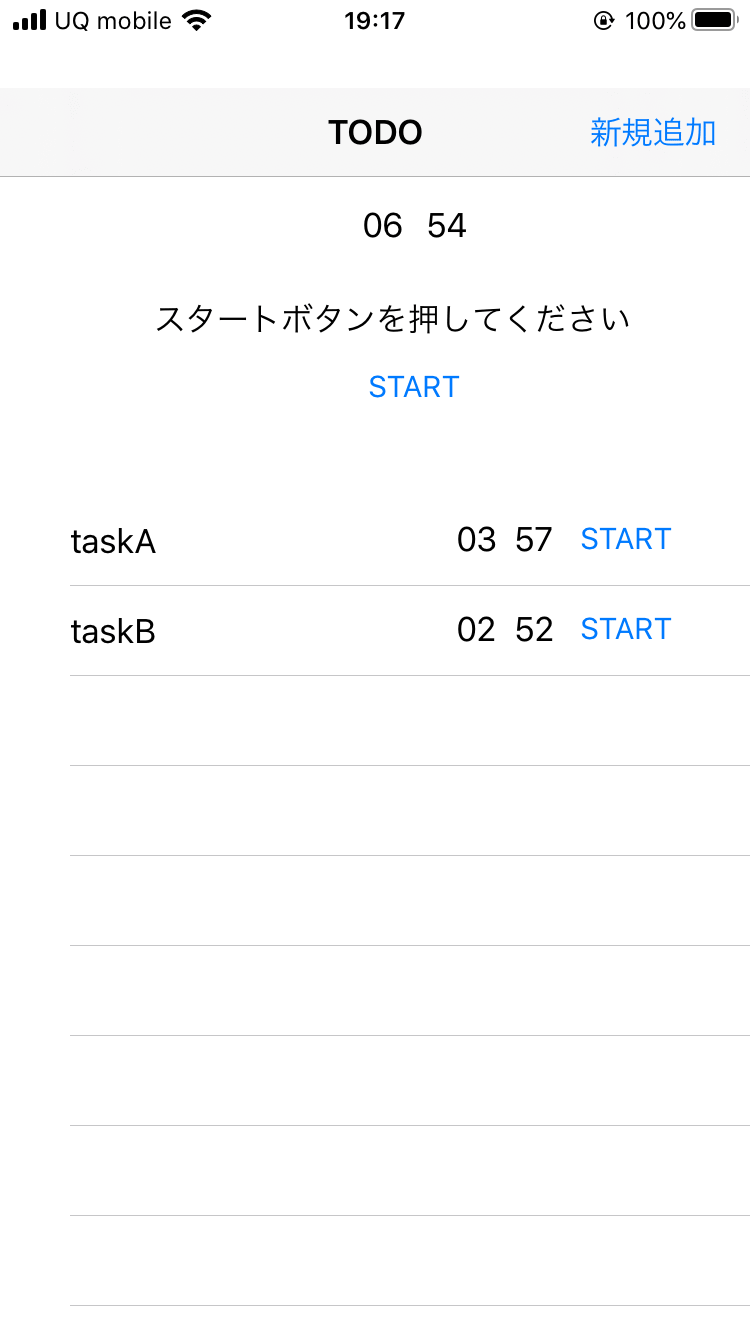
\includegraphics[width=5cm]{images/3/yobi.png}}
		\caption{使用アプリケーション}
		\label{fig:yobiapp}
	\end{center}
  	\end{minipage}
	
\end{tabular}
\end{center}
\end{figure}

\begin{table}[htb]
\begin{center}
  \caption{被験者に対する質問項目}
  \begin{tabular}{|l|l|} \hline
   1 & 支度開始時刻 \\ \hline
   2 & 外出時刻 (理想時刻,外出時刻のタイムリミット) \\ \hline
   3 & 必要タスク \\ \hline
   4 & タスク別所要時間 \\ \hline
  \end{tabular}
  \label{tb:Q}
\end{center}
\end{table}

\subsection{実験結果}
計測日数が0日だった6名(内時間管理に苦手意識のある被験者は5名)を分析対象から除外し,
有効回答者3名(内時間管理に苦手意識のある被験者は1名)を分析の対象とした.
以後被験者A,B,C,と供述する.被験者データとしては被験者Aのみ苦手意識があり.被験者Bのみ3日間,それ以外が1日間のデータが得られた.
図~\ref{fig:re1},\ref{fig:re2}は横軸を被験者名,縦軸を予測時間と実際の時間の差分を可視化したものである.
日常生活動作において被験者A,B,Cは最大3分以上認識の誤差が生じていた.両者グループを比較した際は,Aの方がより誤差の範囲が大きかった.
\begin{figure}[ht]
\begin{center}
\begin{tabular}{c}

	\begin{minipage}[b]{0.5\linewidth}
	\begin{center}
		\fbox{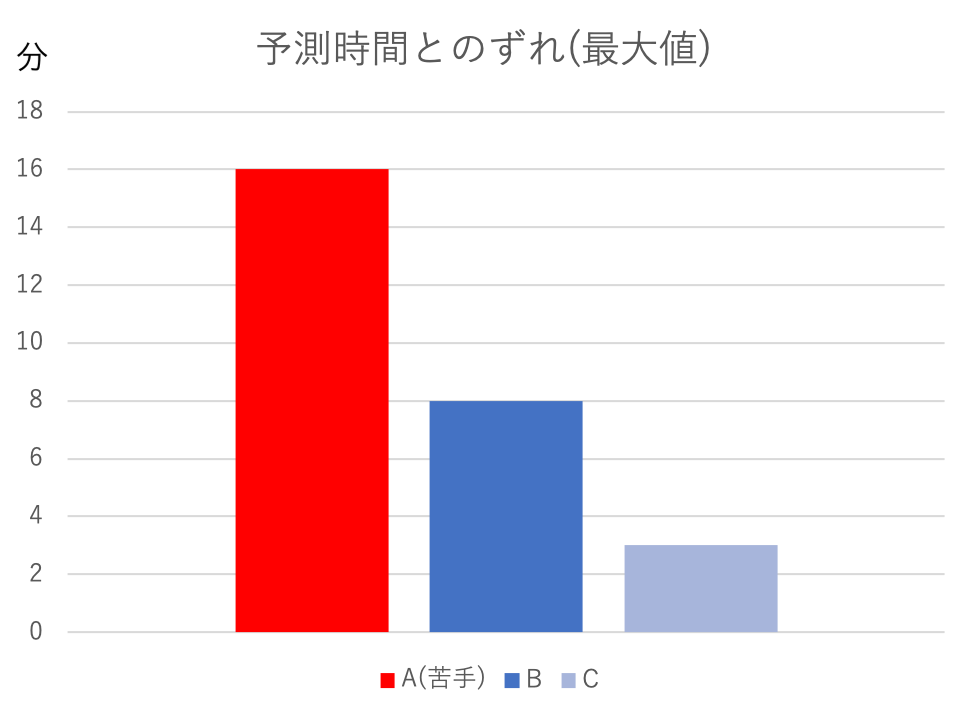
\includegraphics[width=8cm]{images/3/1.png}}
		\caption{被験者結果(最大値)}
		\label{fig:re1}
	\end{center}
  	\end{minipage}
	
		\begin{minipage}[b]{0.5\linewidth}
	\begin{center}
		\fbox{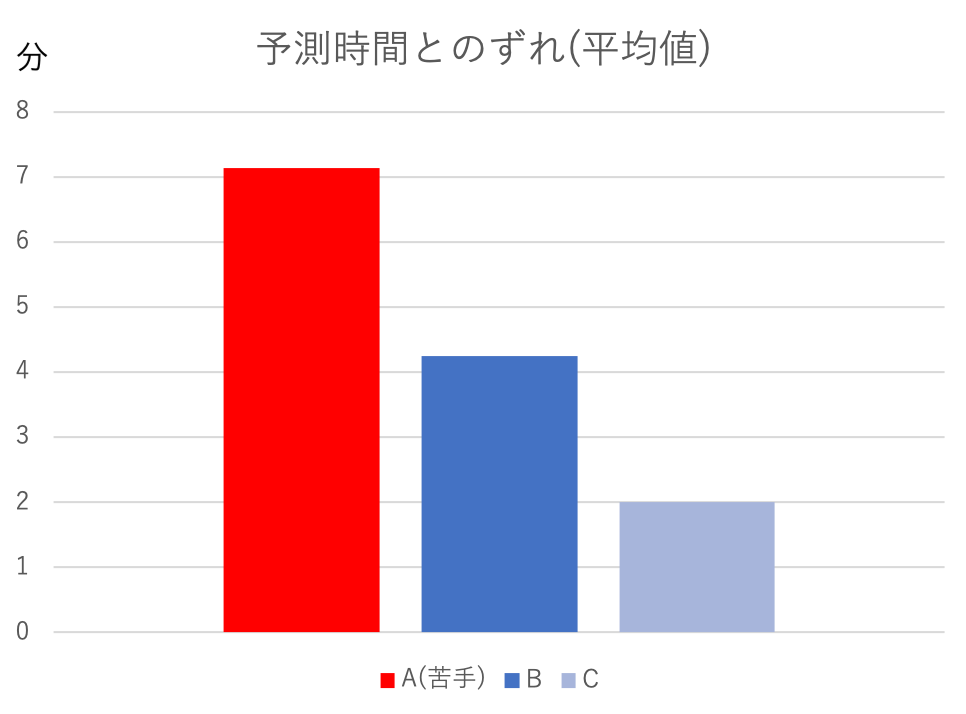
\includegraphics[width=8cm]{images/3/2.png}}
		\caption{被験者結果2}
		\label{fig:re2}
	\end{center}
  	\end{minipage}

\end{tabular}
\end{center}
\end{figure}

また,被験者によっては時間の計画の時点から不備が発生している日もあった.Bにおいては日常生活動作毎の予測時間の合計が予想準備時間(支度開始見込み時刻 - 第一理想時刻)を超えており,計画面から間に合わない計画を立てていた.(事実その日は第一理想時刻には間に合わず,第一理想時刻と第二理想時刻の間に外出していた.)また,それぞれの日常生活動作の内訳は以下の通りである.

\begin{figure}[hb]
	\begin{center}
	\fbox{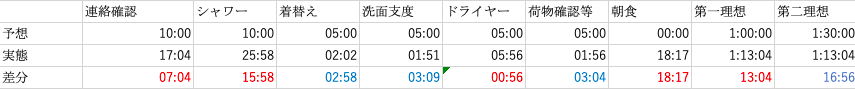
\includegraphics[width=12cm]{images/3/A.png}}
		\caption{被験者Aの内訳}
		\label{fig:top_point}
	\end{center}
\end{figure}

\begin{figure}[hb]
	\begin{center}
	\fbox{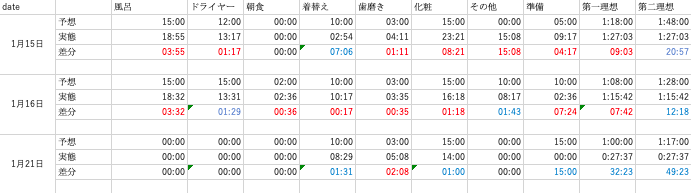
\includegraphics[width=12cm]{images/3/B.png}}
		\caption{被験者Bの内訳}
		\label{fig:top_point}
	\end{center}
\end{figure}

\begin{figure}[hb]
	\begin{center}
	\fbox{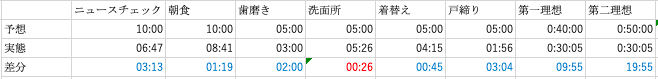
\includegraphics[width=12cm]{images/3/C.png}}
		\caption{被験者Cの内訳}
		\label{fig:top_point}
	\end{center}
\end{figure}

\section{狙い}
3.2で行った実験の結果から,「逆算が苦手」の定義は複数人規模のプロジェクト管理でも言及されていた事と同様に,各タスク見込み時間を実態より短く認識している「見積もり時間の誤差の大きさ」場合とタスク見込み時間の総時間と総準備時間の認識が合致していない上に不十分な予備時間の確保である「バッファの不備」が原因である場合が考えられる.更に破綻したデータは苦手意識のないグループで発見された為,本人の苦手意識にか関わらず被験者の時間管理能力を把握していく必要があると考えられる.
一方で,本予備実験においては被験者数・有効データ数共に少なく,更なる実験が必要であると考えられる.

本研究では,「逆算が苦手」の定義をデータを用いて更なる分析を進めると共に,主要な原因であると考えられる時間管理の見積もり精度に起因された逆算の甘さをiOSアプリケーションを用いて補正する事で時間管理に関する心理的負荷及び逆算精度の改善を図る.